\documentclass[
  bibliography=totoc,     % Literatur im Inhaltsverzeichnis
  captions=tableheading,  % Tabellenüberschriften
  titlepage=firstiscover, % Titelseite ist Deckblatt
]{scrartcl}

% Paket float verbessern
\usepackage{scrhack}

% Warnung, falls nochmal kompiliert werden muss
\usepackage[aux]{rerunfilecheck}

% unverzichtbare Mathe-Befehle
\usepackage{amsmath}
% viele Mathe-Symbole
\usepackage{amssymb}
% Erweiterungen für amsmath
\usepackage{mathtools}

% Fonteinstellungen
\usepackage{fontspec}
% Latin Modern Fonts werden automatisch geladen
% Alternativ:
%\setromanfont{Libertinus Serif}
%\setsansfont{Libertinus Sans}
%\setmonofont{Libertinus Mono}
\recalctypearea % Wenn man andere Schriftarten gesetzt hat,
% sollte man das Seiten-Layout neu berechnen lassen

% deutsche Spracheinstellungen
\usepackage{polyglossia}
\setmainlanguage{german}


\usepackage[
  math-style=ISO,    % ┐
  bold-style=ISO,    % │
  sans-style=italic, % │ ISO-Standard folgen
  nabla=upright,     % │
  partial=upright,   % ┘
  warnings-off={           % ┐
    mathtools-colon,       % │ unnötige Warnungen ausschalten
    mathtools-overbracket, % │
},                       % ┘
]{unicode-math}

% traditionelle Fonts für Mathematik
\setmathfont{Latin Modern Math}
% Alternativ:
%\setmathfont{Libertinus Math}

\setmathfont{XITS Math}[range={scr, bfscr}]
\setmathfont{XITS Math}[range={cal, bfcal}, StylisticSet=1]

% Zahlen und Einheiten
\usepackage[
locale=DE,                   % deutsche Einstellungen
separate-uncertainty=true,   % immer Fehler mit \pm
per-mode=symbol-or-fraction, % / in inline math, fraction in display math
]{siunitx}

% chemische Formeln
\usepackage[
version=4,
math-greek=default, % ┐ mit unicode-math zusammenarbeiten
text-greek=default, % ┘
]{mhchem}

% richtige Anführungszeichen
\usepackage[autostyle]{csquotes}

% schöne Brüche im Text
\usepackage{xfrac}

% Standardplatzierung für Floats einstellen
\usepackage{float}
\floatplacement{figure}{htbp}
\floatplacement{table}{htbp}

% Floats innerhalb einer Section halten
\usepackage[
section, % Floats innerhalb der Section halten
below,   % unterhalb der Section aber auf der selben Seite ist ok
]{placeins}

% Seite drehen für breite Tabellen: landscape Umgebung
\usepackage{pdflscape}

% Captions schöner machen.
\usepackage[
  labelfont=bf,        % Tabelle x: Abbildung y: ist jetzt fett
  font=small,          % Schrift etwas kleiner als Dokument
  width=0.9\textwidth, % maximale Breite einer Caption schmaler
]{caption}
% subfigure, subtable, subref
\usepackage{subcaption}

% Grafiken können eingebunden werden
\usepackage{graphicx}
% größere Variation von Dateinamen möglich
\usepackage{grffile}

% schöne Tabellen
\usepackage{booktabs}

% Verbesserungen am Schriftbild
\usepackage{microtype}

% Literaturverzeichnis
\usepackage[style=alphabetic,]{biblatex}
% Quellendatenbank
\addbibresource{lit.bib}

% Hyperlinks im Dokument
\usepackage[
  unicode,        % Unicode in PDF-Attributen erlauben
  pdfusetitle,    % Titel, Autoren und Datum als PDF-Attribute
  pdfcreator={},  % ┐ PDF-Attribute säubern
  pdfproducer={}, % ┘
]{hyperref}
% erweiterte Bookmarks im PDF
\usepackage{bookmark}

% Trennung von Wörtern mit Strichen
\usepackage[shortcuts]{extdash}

\title{V303: Lock-In-Verstärker}
\author{
  Simon Schulte
  \texorpdfstring{
    \\
    \href{mailto:simon.schulte@udo.edu}{simon.schulte@udo.edu}
  }{}
  \texorpdfstring{\and}{, }
  Tim Sedlaczek
  \texorpdfstring{
    \\
    \href{mailto:tim.sedlaczek@udo.edu}{tim.sedlaczek@udo.edu}
  }{}
}
\publishers{TU Dortmund – Fakultät Physik}

\date{Durchführung: 13.12.2016\\
      Abgabe: 20.12.2016}


\begin{document}

\maketitle
\thispagestyle{empty}
\tableofcontents
\newpage
\section{Zielsetzung}
\label{sec:zielsetzung}
Ziel des Versuchs ist es, die Funktionsweise eines Lock-In-Verstärkers
kennenzulernen.
\section{Theorie}
\label{sec:theorie}
Ein Lock-In-Verstärker ist ein Verstärker, dessen Hauptaufgabe darin liegt,
stark verrauschte Signale auf die gesuchte Frequenz zu filtern, wie bei einem
Bandpass. Der Lock-In-Verstärker hat allerdings eine um den Faktor 100 bessere
Güte als ein üblicher Bandpass.
Ein Lock-In-Verstärker moduliert ein Messsignal mit einer Referenzfrequenz
$\omega_0$. Dabei werden das Nutzsignal $U_{sig}$ und das Referenzsignal
$U_{ref}$ in einem Mischer miteinander multipliziert. Dies ist in Abbildung
\ref{fig:V3033} zu sehen. Anschließend integriert der dem Mischer nachgeschaltete
Tiefpass das Mischsignal $U_{sig}\,\times\,U_{ref}$ über mehrere Perioden der
Modulationsfrequenz. Durch die Perioden mitteln sich die unerwünschten
Rauschbeträge weitesgehend heraus. Am Ausgang ist nun eine zur Eingangsspannung
$U_{sig}$ proportionale Gleichspannung $U_{out}\,\propto\,U_0\,\cos\phi$ zu
messen. Dabei ist $\phi$ die veränderliche Phasenlage des Referenzsignals, die
mit dem Nutzsignal $U_{sig}$ synchronisiert wird.
\begin{figure}[htb]
  \centering
  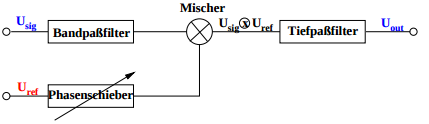
\includegraphics[width=0.8\textwidth]{V3033.png}
  \caption{Schematische Darstellung eines Lock-In-Verstärkers}
  \label{fig:V3033}
\end{figure}
\newpage
In Abbildung \ref{fig:V3034} sind die Signalverläufe für eine sinusförmige
Signalspannung zu sehen, wie sie auch in diesem Versuch vorkommen. Die
Signalspannung ist dabei
\begin{equation}
  U_{sig}\,=\,U_0\,\sin({\omega\,t})
\end{equation}
\label{eqn:1}
Diese wird durch eine Rechteckspannung $U_{ref}$ derselben Spannung moduliert.
$U_{ref}$ ist dabei ein Schalter oder ein Chopper. Man kann $U_{ref}$ durch
eine Fourierreihe nähern. Dann enthält das Produkt aus $U_{sig}$ und $U_{ref}$

\begin{equation}
  U_{out}\,=\,\frac{2}{\pi}U_0
\end{equation}
\label{eqn:2}
Mit einer Phasendifferenz $\phi$ zwischen Nutz- und Referenzspannung wird
\ref{eqn:2} zu
\begin{equation}
  U_{out}\,=\,\frac{2}{\pi}U_0\cos(\phi)
\end{equation}
\label{eqn:3}
Da die Cosinus-funktion maximal wird, wenn das Argument 0 (oder einem Vielfachen
von $2\,\pi$) entspricht, wird die Ausgangsspannung maximal für $\phi$\,=\,0,
also wenn es keinen Phasenunterschied zwischen Nutz- und Referenzspannung gibt.
\begin{figure}[htb]
  \centering
  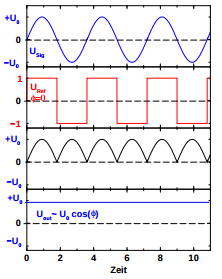
\includegraphics[width=0.5\textwidth]{V3034.png}
  \caption{Signalverläufe für eine sinusförmige Signalspannung}
  \label{fig:V3034}
\end{figure}
\newpage
\section{Durchführung}
\label{sec:durchführung}
\subsection{Versuchsaufbau}
\label{sec:aufbau}
\begin{figure}[htb]
  \centering
  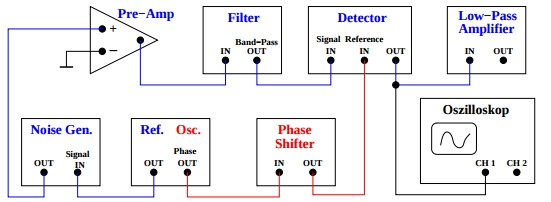
\includegraphics[width=0.9\textwidth]{V3031.png}
  \caption{Schaltplan eines Lock-In-Verstärkers}
  \label{fig:V3031}
\end{figure}
In Abbildung \ref{fig:V3031} ist der Schaltplan eines Lock-In-Verstärkers zu
sehen. Als erstes wurde dieser Schaltplan aufgebaut. Der Schaltplan eines
Lock-In-Verstärkers beinhaltet einen Vorverstärker, die Hoch-, Tief-, und
Bandpassfilter, der Phasenschieber, ein Funktionsgenerator, ein Rauschgenerator,
ein Tiefpass-Verstärker und einen Amplituden-/Lock-In-Detektor. All diese Geräte
sind seperat bedienbar. Dabei verstärkt der Vorverstärker das zu untersuchende
Signal. Die Filter sind dafür da, die gewünschten Frequenzen aus dem Signal
herausszufiltern. Mit dem Phasenschieber kann man das bereits in der Theorie
erwähnte \ref{sec:theorie} $\phi$ variieren. Der Funktionsgenerator wird zum
Erzeugen periodischer elektrischer Signale genutzt.
Der Rauschgenerator erzeugt Rauschen als zufällige Signalschwankung.
\subsection{Versuchsdurchführung}
\label{sec:versuchsdurchführung}
Zuerst werden Messungen ohne Rauschsignal aufgenommen. Dabei wird der
Noise-Generator noch nicht eingeschaltet. Als nächstes wird ein Sinussignal $U_{sig}$
erzeugt mit \SI{1}{kHz} und \SI{5}{mV} (?). Dabei entsteht auch ein Referenzsignal
$U_{ref}$ mit gleicher Frequenz wie $U_{sig}$. Die Ausgangsspannung $U_{out}$
wird dann 5 mal (?) in Abhängigkeit von der Phasenverschiebung bestimmt, nach
der Integration über den Tiefpass, nachdem über den Tiefpass integriert wird.
Danach wird der Noise-Generator eingeschaltet. Die Messungen werden wiederholt.
Als letztes wird noch ein Photo-Detektor in den Schaltplan integriert. Dieser
Schaltplan ist in \ref{fig:V3032} zu sehen. Die LED des Photo-Detektors blinkt
mit \SI{200}{Hz}. Sie kann mit einer Reckteckspannung moduliert werden.
Dann wird als Funktion des Abstandes zwischen LED und Photodiode die
Lichtintensität gemessen und der maximale Abstand $r_{max}$ bestimmt, bei dem
das Licht der LED die Photodiode noch erreicht.
Durch ein Oszilloskop werden die in der Auswertung genutzten Bilder gespeichert.
Dies ist mit Hilfe des "print"-Knopfes am Oszilloskop möglich.
Mit diesem Speicher-Oszilloskop können die Signale aller Komponenten einzeln
vermessen und skizziert werden.

\begin{figure}[htb]
  \centering
  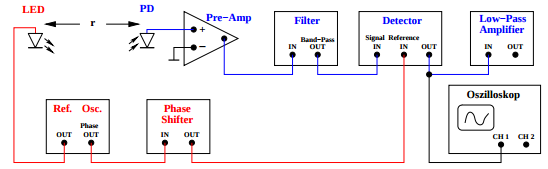
\includegraphics[width=0.5\textwidth]{V3032.png}
  \caption{Schaltplan eines Lock-In-Verstärkers mit einem Photo-Detektor}
  \label{fig:V3032}
\end{figure}

\newpage
\section{Auswertung}
\label{sec:auswertung}
\end{document}
